% Overleaf: main document = main.tex; XeLaTeX is recommended.
% The pdfLaTeX fallback also supports the Chinese text in this report.
\documentclass[conference,a4paper]{IEEEtran}
\usepackage{iftex}
\ifPDFTeX
  \usepackage[T1]{fontenc}
  \usepackage[utf8]{inputenc}
  \usepackage{CJKutf8}
\else
  \ifXeTeX
    \usepackage{xeCJK}
    \setCJKmainfont{FandolSong-Regular}
  \else
    \usepackage[UTF8,scheme=plain,fontset=fandol]{ctex}
  \fi
  \setmainfont{TeX Gyre Termes}
\fi
\usepackage{amsmath,amssymb}
\usepackage{graphicx}
\usepackage{url}
\usepackage[hidelinks]{hyperref}
% Compact float spacing; retain IEEE text size and page margins.
\setlength{\textfloatsep}{4pt plus 1pt minus 1pt}
\setlength{\dbltextfloatsep}{4pt plus 1pt minus 1pt}
\setlength{\floatsep}{4pt plus 1pt minus 1pt}
\setlength{\dblfloatsep}{4pt plus 1pt minus 1pt}
% Compact displayed equations without changing text size or margins.
\AtBeginDocument{%
  \setlength{\abovedisplayskip}{6pt plus 1pt minus 1pt}%
  \setlength{\belowdisplayskip}{6pt plus 1pt minus 1pt}%
  \setlength{\abovedisplayshortskip}{3pt plus 1pt minus 1pt}%
  \setlength{\belowdisplayshortskip}{3pt plus 1pt minus 1pt}%
}
\renewcommand{\refname}{References}
\title{House Price Prediction with Frozen Visual Features and Kernel Fusion}
\author{\IEEEauthorblockN{Shifeng Chen \qquad Haoxuan Ying}
\IEEEauthorblockA{1686631 \qquad 1255329\\
COMP90086 Computer Vision, The University of Melbourne}}
\begin{document}
\ifPDFTeX
\begin{CJK*}{UTF8}{gbsn}
\fi
\maketitle
\raggedbottom

\section{Introduction}
The selling price of a house is usually influenced by multiple factors, such as the size of the house, geographical location, market conditions, decoration materials, etc. However, the feasibility of inferring prices based on one-sided information from photos still needs further discussion. This project aims to study how to use computer vision to predict housing prices based on this incomplete visual information through comparative experiments and ablation experiments.

The experiment uses SIFT and a bag of visual words to determine whether local appearance is helpful for prediction, and then compares the training settings, data augmentation, and network structure of AlexNet~\cite{alexnet} item by item. Afterwards, we further used frozen pre-trained features from CLIP~\cite{clip}, SigLIP2~\cite{siglip2}, and Perception Encoder~\cite{pe} to examine whether preserving the entire image information, adjusting features, and regression methods could reduce errors, and finally tested whether combining different models was better than the strongest single model.

\section{Methods}
\subsection{Data, Metrics, and Evaluation Methods}
The dataset contains 8,000 labeled images and 3,000 unlabeled test images containing houses in Southern California, with house prices in thousands of US dollars. The regression of housing prices only uses images and labels provided by the course for training, and pre-trained encoders are used to extract general visual features.

We divided the labeled data into 6,399 training images and 1,601 validation images using seed 2026. We group identified duplicate or related images into the same training/validation set. For fair comparison, we always use the same data partitioning when changing training seeds. For $N$ evaluation images, assuming the true price is $y_i$ and the predicted price is $\hat y_i$:
\begin{equation}
\mathrm{MSE}=\frac{1}{N}\sum_{i=1}^{N}(\hat y_i-y_i)^2,\qquad
\mathrm{MAE}=\frac{1}{N}\sum_{i=1}^{N}|\hat y_i-y_i|.
\end{equation}
We use MSE (Mean Squared Error) as the main indicator, and MAE (Mean Absolute Error) as an auxiliary reference, with units of (thousand US dollars)$^2$ and thousand US dollars, respectively.

We selected seeds 2026, 2027, and 2028 for comparison. Only when the mean MSE decreases and at least two seeds improve can the improvement effect of the method be recognized. Frozen-feature regressors use grouped three-fold out-of-fold (OOF) predictions for parameter selection. Standardization, PCA, and supervised transformations are learned only in the corresponding fitting fold. The SIFT dictionary and its standardizer only use the training set for fitting.

\subsection{Baseline and CNN Controlled Experiments}
We calculate the average housing price in the training set as a constant prediction reference. Use traditional methods to extract grayscale SIFT descriptors~\cite{sift1999,sift}, aggregate them into 256 'visual words'~\cite{bovw}, and count word frequencies. After L1 normalization, square root transformation, L2 normalization, and standardization, the histogram is input into ridge regression~\cite{ridge} ($\alpha=10$). The bag of words weakens the spatial arrangement of images, so it is necessary to introduce additional CNN learning space combinations.

The AlexNet-style network~\cite{alexnet} is trained from random weights, using five convolutional layers and a fully connected regression head of 9216--4096--4096--1. The image is directly scaled to $224\times224$ without filtering. After converting pixel values to $[0,1]$, we normalize the RGB channels with a mean and standard deviation of 0.5. We use AdamW~\cite{adamw} as the optimizer, with a learning rate and weight decay of $10^{-4}$, and dropout~\cite{dropout2012,dropout} of 0.5.

Due to local memory limitations, only 4 images are used per batch, accumulating 8 training batches of gradients. A total of 40--60 rounds of training were conducted, with 15 rounds of early stopping patience and a relative improvement threshold of 0.1\%. Finally, the checkpoint with the lowest MSE was used for validation.

we first test changes to the learning rate, effective batch size, and dropout separately. We also test Adam~\cite{adam}, cosine learning-rate decay without restarts~\cite{sgdr}, and different weight initializations~\cite{xavier,heinit}. Geometric and degradation augmentations are tested separately. For horizontal flipping, the probability is 0.5. Augmentation and dropout are disabled during validation.

Architecture comparison includes: replacing the second $5\times5$ convolution with two $3\times3$ convolutions~\cite{vgg}, Inception style multi-scale module~\cite{inception}, and projection residual connection~\cite{resnet}. To verify if the prediction head is too large, we also projected the $6\times6$ grid features onto 128 dimensions and added positional and normalization processing. We replaced the fully connected head with mean pooling and linear regression. Also test single-layer Transformer~\cite{transformer}, set to 128 dimensional, four head attention, and 512 dimensional feedforward layer. Each item was compared with its corresponding control.

Brightness and contrast were used as additional experiments, and seed 2026 was screened separately. Before scaling and normalization, a $U(0.9,1.1)$ magnification was applied without adding any other enhancements. We use same initialization, partitioning, and training settings with the newly trained non enhanced AlexNet, and do not directly pair and compare with earlier batches.

\subsection{Frozen Representations, Multi-view and Regression}
Encoder weights are kept frozen, and only the price regression is learned. Using CLIP ViT-B/32 features combined with standardization and ridge regression as a reference; ultimately using SigLIP2 So400m NaFlex, PE-Core-L/14 and PE-Core-G/14. NaFlex preserves the aspect ratio, uses 576 patches, and outputs 1,152-dimensional features.

To retain edge content that might be lost during official cropping, an all-proportion scaling and gray padding full-image view is added. PE-L combines official preprocessing, 336-pixel padded full-image and central cropping preserving 60\% of the original aspect ratio; PE-G combines the official 448-pixel view with padded full-image. Each view's features are L2 normalized separately, then concatenated and normalized again to obtain 3,072-dimensional PE-L and 2,560-dimensional PE-G features.

RBF kernel ridge regression~\cite{krr} learns price prediction based on feature similarity. Let $x_i$ be the unitized features, $y$ be the fitted sample prices, and $\bar y$ be their mean, then

\begin{equation}
 K_{ij}=\exp(-\gamma\|x_i-x_j\|^2),\quad
 c=(K+\alpha I)^{-1}(y-\bar y\mathbf{1}).
\end{equation}
Prediction is $\bar y+k(x)^Tc$, where $k(x)$ is the kernel similarity vector between the new image and the fitted samples, and negative predictions are truncated to zero. $\gamma$ controls the distance scale of similarity, and $\alpha$ controls regularization. We search $\gamma\in\{1,4,16\}$ and $\alpha\in\{0.01,0.1,1,10\}$ within each fold, with NaFlex selecting $\gamma=1$ and $\alpha=0.1$.

PE-L employs partial least squares (PLS)~\cite{pls1966,pls} to incorporate price-related directions because visual similarity can not be treated as price proximity. In each fitted fold, the model learns 16 components, and the first four standardized scores $s$ are used to construct the kernel:
\begin{equation}
 k(x,x')=\exp\left(-\|x-x'\|^2-0.1\frac{\|s-s'\|^2}{4}\right),
\end{equation}
where $\alpha=1$.

PE-G uses PCA~\cite{pca} to compress features without relying on price information, comparing 64, 256, and 1,024 dimensions, with whitening powers of 0 or 0.5, followed by L2 normalization. Compression changes distances, so we compare the fixed $\gamma=4$ with the following bandwidth calibration:
\begin{equation}
 \gamma'=4\frac{\operatorname{median}\|x_i-x_j\|^2}
 {\operatorname{median}\|z_i-z_j\|^2}.
\end{equation}
where $z$ is the unit vector after transformation. Each fitted fold fixed the seed to draw 8,192 pairs of candidate images, calculate the median after removing self-pairs, without using hold-out folds or price information. The final selection is the unwhitened PCA256 with $\alpha=1$.

\subsection{Ensemble and Final Refitting}
We combine models using stacking regression~\cite{stacking} to make use of their different predictions. The weights are learned from OOF predictions, are non-negative, and sum to one. We divide the OOF records into three folds and rotate the held-out fold, learning weights on two folds and evaluating on the remaining fold (meta-CV). We retain a new branch only if adding it reduces meta-CV MSE by more than 1\% compared with the existing ensemble, lowers MSE in at least two of the three folds, and reduces validation MSE. The base models have already been selected, and the validation set has been used repeatedly, so these scores are not fully independent test results.

The final weights are NaFlex 0.108065, PE-L PLS 0.080806, and PE-G PCA 0.811129. We keep these ensemble weights and the selected configurations fixed, then refit the transformations and regression heads on all 8,000 labeled images. For the PCA branch, the RBF kernel bandwidth is recalculated from these images using the same calibration rule. We then predict prices for the 3,000 test images. Test labels are not used for training or hyperparameter selection.

\section{Results}
% Native two-column IEEE table; no additional LaTeX package required.
\begin{table*}[t]
\centering
\caption{Representative configurations evaluated on the fixed validation split.}
\label{tab:representative-results}
\small
\setlength{\tabcolsep}{4pt}
\renewcommand{\arraystretch}{1.0}
\begin{tabular*}{\textwidth}{@{\extracolsep{\fill}}lcr@{\,}c@{\,}rr@{}}
\hline
Method & Seeds & \multicolumn{3}{c}{Validation MSE} & Validation MAE \\
\hline
AlexNet (no augmentation) & 3 & 127,774 & $\pm$ & 486 & 264.52 \\
AlexNet (Adam, lr=0.001) & 3 & 128,284 & $\pm$ & 1,106 & 264.80 \\
AlexNet + horizontal flip & 3 & 126,810 & $\pm$ & 1,902 & 268.02 \\
Flip AlexNet + small-kernel stack & 1 & 127,320 &  &  & 262.19 \\
Flip AlexNet + mean-pooling head & 3 & 122,334 & $\pm$ & 1,589 & 261.48 \\
Mean-pooling head + Transformer & 1 & 124,389 &  &  & 259.55 \\
Frozen CLIP B32 + Ridge & -- & 91,821 &  &  & 223.27 \\
Frozen PE-G, two views + PCA/KRR & -- & 52,806 &  &  & 160.67 \\
\textbf{Selected three-encoder fusion} & \textbf{--} & \textbf{52,201} & \textbf{} & \textbf{} & \textbf{159.58} \\
\hline
\end{tabular*}
\par\smallskip
\begin{minipage}{0.96\textwidth}
\scriptsize
Validation $n=1{,}601$. MSE: (thousand USD)$^2$; MAE: thousand USD.
Three-seed results report MSE mean $\pm$ sample SD and MAE mean.
Single-seed results use seed 2026; -- indicates frozen-feature evaluation.
\end{minipage}
\end{table*}

\begin{figure*}[t]
\centering
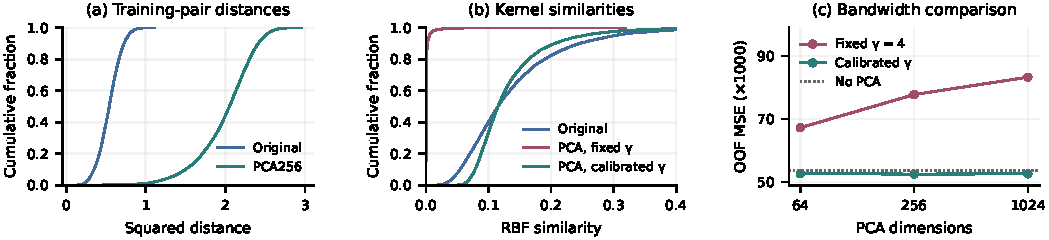
\includegraphics[width=0.82\textwidth]{figures/report_pca_distance_bandwidth_oof.pdf}
\caption{PE-G diagnostics. (a, b) Empirical cumulative distributions of distances and kernel similarities for 8,192 training pairs; (c) grouped three-fold OOF MSE for unwhitened PCA. Transforms and bandwidths are fitted within each fold. Panel (b) shows similarities from 0 to 0.4.}
\label{fig:pca-zh}
\end{figure*}
\begin{figure}[t]
\centering
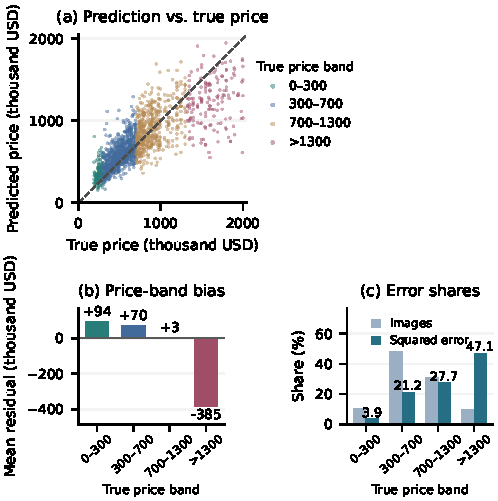
\includegraphics[width=0.76\columnwidth]{figures/report_prediction_scatter_price_band_errors.pdf}
\caption{Final ensemble on 1,601 validation images. (a) Predicted versus true prices; the dashed line indicates perfect predictions and colors match the price bands in (b). (b) Mean residual $\hat y-y$. (c) Shares of samples and squared error. Price bands: $(0,300]$, $(300,700]$, $(700,1300]$, and above 1,300 thousand USD.}
\label{fig:errors-zh}
\end{figure}
\begin{figure*}[t]
\centering
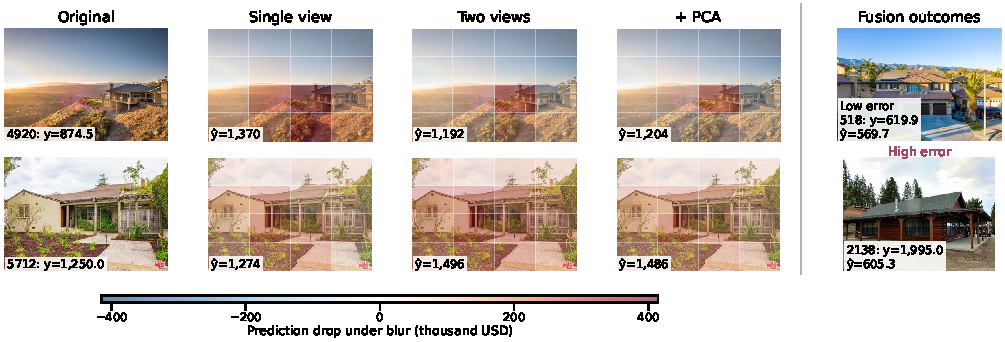
\includegraphics[width=0.82\textwidth]{figures/report_regional_and_outcome_cases.pdf}
\caption{Left four columns: $4\times4$ blur-replacement sensitivity for PE-G single-view, two-view and PCA models. Red/blue indicates a prediction decrease/increase, with a shared scale. Cases 4920/5712 show the largest improvement/deterioration from adding the full-image view among 1,543 landscape validation images. Right: separate final-ensemble cases, 518 at the 25th percentile of absolute error and 2138 as a fixed failure case. Prices are in thousand USD.}
\label{fig:occlusion-zh}
\end{figure*}


\subsection{Comparison of average price, SIFT, and AlexNet baseline}
The MSE for the base of the training average price prediction is 151,839.69. SIFT--BoVW--Ridge extracts appearance features to obtain price-related signals, reducing them to $145,336.73\pm1,091.58$. Considering that bagager summaries lose spatial arrangement, we further test CNNs capable of learning feature combinations. Using the AlexNet patch, the final average MSE is 128,415.68, which drops to 127,774.42 after direct scaling (Table~\ref{tab:representative-results-zh}). At this point, attribution analysis reveals that the source of residual error may come from training methods or model size.

\subsection{CNN Training, Data Augmentation, and Architecture Ablation}
\begin{table}[t]
\centering
\caption{AlexNet augmentation comparisons.}
\label{tab:augmentation-zh}
\small
\setlength{\tabcolsep}{3pt}
\begin{tabular*}{\columnwidth}{@{\extracolsep{\fill}}lrr@{}}
\hline
Setting & MSE & MAE \\
\hline
\multicolumn{3}{l}{\emph{A. Geometric and degradation screen}} \\
No augmentation & 128,268.67 & 259.99 \\
Horizontal flip & 126,601.97 & 263.16 \\
Rotation & 129,526.18 & 260.29 \\
Translation & 129,162.73 & 262.97 \\
Random crop & 130,222.98 & 272.60 \\
Gaussian blur & 129,941.36 & 261.20 \\
Gaussian noise & 131,174.53 & 271.48 \\
Random erasing & 128,114.40 & 268.07 \\
\multicolumn{3}{l}{\emph{B. Photometric screen}} \\
Fresh control & 131,389.94 & 282.64 \\
Brightness & 131,433.91 & 274.50 \\
Contrast & 128,860.53 & 269.01 \\
\hline
\end{tabular*}
\par\smallskip
\begin{minipage}{\columnwidth}\scriptsize
Seed 2026; validation n=1,601. One augmentation per run; A and B use their respective unaugmented controls.
\end{minipage}
\end{table}

Hyperparameter tuning and data augmentation in same-seed control experiments didn't show noticeable results. Adam with a learning rate of 0.001 only improved with seed 2026; cosine decay, alternative batch sizes, and lower dropout also didn’t pass the retention criteria. For data augmentation, horizontal flipping reducing the average MSE by 964.41, but MAE increased from 264.52 to 268.02. Erasing showed improvement in the initial screening, but only won once in three pairwise checks, so it was dropped.


Next, in terms of architecture, to check whether a large prediction head limits learning, we replaced it with mean pooling, then MSE decrease by 4,475.78 compared to flipped AlexNet. Small kernels, multi-scale, and residual pre-screening didn't outperform the baseline; for Transformer, the MSE of a single seed increased by 3,615.11 compared to the compact head. So, we found that increasing capacity doesn't solve the prediction difficulty under current conditions.

Table~\ref{tab:augmentation-zh} summarizes the initial screening of single seeds. Overall MSE for contrast improved by 1.93\%, but for the tail above 1,300, MSE worsened by 17.14\%; brightness made the tail MSE worse by 3.86\%. Observation shows that a drop in average error can still come with setbacks in high-value predictions.

\begin{table}[t]
\centering
\caption{Fusion ablation and strongest-branch comparison.}
\label{tab:fusion-ablation-zh}
\small
\setlength{\tabcolsep}{3pt}
\begin{tabular*}{\columnwidth}{@{\extracolsep{\fill}}lrr@{}}
\hline
Configuration & Val. MSE & Meta MSE \\
\hline
PE-G PCA only & 52,805.77 & 52,531.27 \\
No NaFlex & 52,597.50 & 52,359.30 \\
No PE-L PLS & 52,194.81 & 52,244.24 \\
No PE-G PCA & 57,372.90 & 57,694.20 \\
Equal weights & 53,847.68 & 54,214.33 \\
Full fusion & 52,201.21 & 52,210.22 \\
\hline
\end{tabular*}
\par\smallskip
\begin{minipage}{\columnwidth}\scriptsize
After branch removal, remaining weights are refitted on training OOF predictions only. Validation n=1,601; meta uses three-fold cross-fitting on training OOF predictions.
\end{minipage}
\end{table}




\subsection{Pretrained Features, Multi-View, and Kernel Regression}
Freezing CLIP and combining it with ridge regression achieved an MSE of 91,820.73, pushing the research towards richer transfer visual representations. Using transfer representations allows us to fully leverage the pretrained encoder's ability to extract visual features, reducing the model's burden of learning and predicting from limited price labels.

We extracted features separately from the official PE-G cropped view and the full image view with proportional scaling and gray padding, then concatenated them for regression. After that, the MSE dropped from 55,097.49 to 53,252.81, and the OOF MSE dropped from 55,679.73 to 53,646.46, supporting broader image coverage.


However, using PCA256 to compress features and keeping $\gamma=4$, the OOF MSE worsened to 77,771.43. The median squared distance during training went from 0.5402 to 2.0515, so $\gamma$ was calibrated to 1.05323 (Fig~\ref{fig:pca-zh}). The OOF MSE dropped to 52,531.27, with validation MSE at 52,805.77 and MAE at 160.67. The change in distances lowers the kernel similarity for the same bandwidth, so the downstream similarity scale needs to be adjusted accordingly after compression.



\subsection{Fusion Performance and Branch Ablation}
After adding PE-G PCA, the meta-CV MSE dropped from 53,052.57 to 52,210.22, improving across all three folds; the validation MSE went down from 52,524.78 to 52,201.21; and the public leaderboard MSE changed from 47,837.69 to 47,291.35.

Tab~\ref{tab:fusion-ablation-zh} checks if the fusion surpasses the strongest single branch. Fusion improves over PE-G PCA by 1.14\%; removing PE-G comes at the highest cost, while equal weighting weakens its contribution. After removing PE-L, MSE slightly decreases, but meta-CV worsens, so its benefit is small and depends on the evaluation metric. PE-L contributes little, possibly because its predictions overlap a lot with the dominant PE-G branch.

The final fusion shows a systematic pricing error: the average residual of $+6.51$ hides the overestimation at the low end (up to $+93.72$ when under 300) and underestimation at the high end (down to $-385.16$ when over 1,300). The 159 highest-priced images account for 47.13\% of the squared error (Fig.~\ref{fig:errors-zh}), and the 161 most erroneous images contribute 63.30\%. RMSE is 228.48, and the median absolute error is 113.41.

To examine the effect of visible content, we compare the responses of PE-G single-view, dual-view, and PCA regression heads under $4\times4$ region replacement~\cite{occlusion}. On the left side of Fig~\ref{fig:occlusion-zh}, a blurred replacement with a radius of 8 is used, and in the unified color scale, red indicates that the replacement caused the predicted price to drop.

PCA kept these main response spots: the dual views at 4920 and 5712 have correlation coefficients with the PCA blurred response of 0.915 and 0.977, but the response amplitudes dropped, and the predicted values only changed slightly. This suggests that compression still preserves the main spatial evidence when recalibrating similarity; 

\section{Discussion}
This study mainly explores three approaches to reveal how visual information can inform house valuation. First, there’s the manual SIFT feature route, which allows controlled extraction of key local appearance features. However, summarizing with a visual bag-of-words can easily lose spatial relationships, making it hard to distinguish houses whose value depends on the layout of the building and surrounding environment. 

Next is the CNN model route. This setup can automatically learn features from the data. Controlled experiments showed how optimization, augmentation, and architecture interact with limited labeled data to affect learning. Using a compact prediction head helps match model capacity to available supervision, which might be more effective than just increasing model complexity and may reduce overfitting to accidental image details. Experiments with horizontal flips and contrast adjustments revealed that augmentations need to preserve the information necessary for target predictions: reducing sensitivity to image changes could improve one metric but hurt another.

Finally, the advantage of freezing a pre-trained encoder is that it leverages general visual knowledge, reducing the burden of learning visual representations from scratch with limited house price labels. At the same time, results from multi-view and feature adaptation experiments indicate that prediction depends on which image information is retained and how visual similarity is converted into price relationships. Increasing representation diversity can supplement visual cues but cannot eliminate valuation errors caused by invisible factors like location, size, and transaction conditions. 

Overall, combining the three approaches, this study shows that a single house image contains visual signals useful for valuation, and effectively using these signals requires aligning representation capacity, supervision scale, and regression methods. Rather than endlessly increasing model complexity, the key is retaining relevant features from images and establishing a mapping suited to the task. 


\clearpage
\begin{thebibliography}{99}
\bibitem{alexnet} A. Krizhevsky, I. Sutskever, and G. E. Hinton, ``\href{https://papers.nips.cc/paper_files/paper/2012/hash/c399862d3b9d6b76c8436e924a68c45b-Abstract.html}{ImageNet classification with deep convolutional neural networks},'' \emph{Advances in Neural Information Processing Systems, vol. 25}, 2012.
\bibitem{clip} A. Radford et al., ``\href{https://proceedings.mlr.press/v139/radford21a.html}{Learning transferable visual models from natural language supervision},'' \emph{Proc. ICML}, 2021, pp. 8748--8763.
\bibitem{siglip2} M. Tschannen et al., ``\href{https://arxiv.org/abs/2502.14786}{SigLIP 2: Multilingual vision-language encoders with improved semantic understanding, localization, and dense features},'' \emph{arXiv:2502.14786}, 2025.
\bibitem{pe} D. Bolya et al., ``\href{https://arxiv.org/abs/2504.13181}{Perception Encoder: The best visual embeddings are not at the output of the network},'' \emph{arXiv:2504.13181}, 2025.
\bibitem{sift1999} D. G. Lowe, ``\href{https://www.cs.ubc.ca/~lowe/papers/iccv99.pdf}{Object recognition from local scale-invariant features},'' \emph{Proc. ICCV}, 1999, pp. 1150--1157.
\bibitem{sift} D. G. Lowe, ``\href{https://www.cs.ubc.ca/~lowe/papers/ijcv04.pdf}{Distinctive image features from scale-invariant keypoints},'' \emph{International Journal of Computer Vision, vol. 60}, 2004, pp. 91--110.
\bibitem{bovw} J. Sivic and A. Zisserman, ``\href{https://www.robots.ox.ac.uk/~vgg/publications/2003/Sivic03/}{Video Google: A text retrieval approach to object matching in videos},'' \emph{Proc. ICCV}, 2003, pp. 1470--1477.
\bibitem{ridge} A. E. Hoerl and R. W. Kennard, ``\href{https://doi.org/10.1080/00401706.1970.10488634}{Ridge regression: Biased estimation for nonorthogonal problems},'' \emph{Technometrics, vol. 12}, 1970, pp. 55--67.
\bibitem{adamw} I. Loshchilov and F. Hutter, ``\href{https://arxiv.org/abs/1711.05101}{Decoupled weight decay regularization},'' \emph{Proc. ICLR}, 2019.
\bibitem{dropout2012} G. E. Hinton et al., ``\href{https://arxiv.org/abs/1207.0580}{Improving neural networks by preventing co-adaptation of feature detectors},'' \emph{arXiv:1207.0580}, 2012.
\bibitem{dropout} N. Srivastava et al., ``\href{https://jmlr.org/papers/v15/srivastava14a.html}{Dropout: A simple way to prevent neural networks from overfitting},'' \emph{Journal of Machine Learning Research, vol. 15}, 2014, pp. 1929--1958.
\bibitem{adam} D. P. Kingma and J. Ba, ``\href{https://arxiv.org/abs/1412.6980}{Adam: A method for stochastic optimization},'' \emph{Proc. ICLR}, 2015.
\bibitem{sgdr} I. Loshchilov and F. Hutter, ``\href{https://arxiv.org/abs/1608.03983}{SGDR: Stochastic gradient descent with warm restarts},'' \emph{Proc. ICLR}, 2017.
\bibitem{xavier} X. Glorot and Y. Bengio, ``\href{https://proceedings.mlr.press/v9/glorot10a.html}{Understanding the difficulty of training deep feedforward neural networks},'' \emph{Proc. AISTATS}, 2010, pp. 249--256.
\bibitem{heinit} K. He et al., ``\href{https://openaccess.thecvf.com/content_iccv_2015/html/He_Delving_Deep_into_ICCV_2015_paper.html}{Delving deep into rectifiers: Surpassing human-level performance on ImageNet classification},'' \emph{Proc. ICCV}, 2015, pp. 1026--1034.
\bibitem{vgg} K. Simonyan and A. Zisserman, ``\href{https://arxiv.org/abs/1409.1556}{Very deep convolutional networks for large-scale image recognition},'' \emph{Proc. ICLR}, 2015.
\bibitem{inception} C. Szegedy et al., ``\href{https://openaccess.thecvf.com/content_cvpr_2015/html/Szegedy_Going_Deeper_With_2015_CVPR_paper.html}{Going deeper with convolutions},'' \emph{Proc. CVPR}, 2015, pp. 1--9.
\bibitem{resnet} K. He et al., ``\href{https://openaccess.thecvf.com/content_cvpr_2016/html/He_Deep_Residual_Learning_2016_CVPR_paper.html}{Deep residual learning for image recognition},'' \emph{Proc. CVPR}, 2016, pp. 770--778.
\bibitem{transformer} A. Vaswani et al., ``\href{https://papers.nips.cc/paper_files/paper/2017/hash/3f5ee243547dee91fbd053c1c4a845aa-Abstract.html}{Attention is all you need},'' \emph{Advances in Neural Information Processing Systems, vol. 30}, 2017.
\bibitem{krr} C. Saunders, A. Gammerman, and V. Vovk, ``\href{https://eprints.soton.ac.uk/258942/}{Ridge regression learning algorithm in dual variables},'' \emph{Proc. ICML}, 1998, pp. 515--521.
\bibitem{pls1966} H. Wold, ``Estimation of principal components and related models by iterative least squares,'' \emph{Multivariate Analysis, P. R. Krishnaiah, Ed. Academic Press}, 1966, pp. 391--420.
\bibitem{pls} S. Wold, A. Ruhe, H. Wold, and W. J. Dunn III, ``\href{https://doi.org/10.1137/0905052}{The collinearity problem in linear regression. The partial least squares (PLS) approach to generalized inverses},'' \emph{SIAM Journal on Scientific and Statistical Computing, vol. 5}, 1984, pp. 735--743.
\bibitem{pca} K. Pearson, ``\href{https://doi.org/10.1080/14786440109462720}{On lines and planes of closest fit to systems of points in space},'' \emph{Philosophical Magazine, vol. 2}, 1901, pp. 559--572.
\bibitem{stacking} L. Breiman, ``\href{https://doi.org/10.1007/BF00117832}{Stacked regressions},'' \emph{Machine Learning, vol. 24}, 1996, pp. 49--64.
\bibitem{occlusion} M. D. Zeiler and R. Fergus, ``\href{https://arxiv.org/abs/1311.2901}{Visualizing and understanding convolutional networks},'' \emph{Proc. ECCV}, 2014, pp. 818--833.
\end{thebibliography}

\ifPDFTeX
\end{CJK*}
\fi
\end{document}
